% ============================================================================
% FRONT MATTER
% ============================================================================

% Title page — full-bleed cover defined in main.tex
\bookcover

\cleardoublepage

% Copyright page
\thispagestyle{empty}
\vspace*{\fill}
\begin{center}
    \textbf{IBM watsonx Generative AI Engineer Associate (C1000-185)}\\
    Complete Study Guide \& Exam Workbook\\[1cm]

    Copyright \textcopyright\ \the\year\ by Ruslan Idelfonso Magana Vsevolodovna\\[0.5cm]

    Licensed under the \textbf{Apache License, Version 2.0} (the ``License''); you may not use this work except in compliance with the License. You may obtain a copy of the License at \\
    \url{http://www.apache.org/licenses/LICENSE-2.0}\\[0.5cm]
    Unless required by applicable law or agreed to in writing, this work is distributed on an ``\textsc{as is}'' \textsc{basis, without warranties or conditions of any kind}, either express or implied. See the License for the specific language governing permissions and limitations.\\[1cm]

    \textbf{Independent publication --- no affiliation}\\
    This book is an independent study guide. It is \textbf{not} authored, sponsored, endorsed, or otherwise approved by IBM Corporation, and the author has no commercial relationship with IBM. References to IBM, watsonx, watsonx.ai, watsonx.data, watsonx.governance, Granite, Slate, and InstructLab are made only to describe and prepare candidates for the publicly published \mbox{C1000-185} certification objectives. All such names are trademarks or registered trademarks of IBM Corporation.\\[0.5cm]

    The information in this book is provided for educational and exam-preparation purposes only. Every effort has been made to align the content with the publicly available C1000-185 study guide and the current watsonx.ai API documentation. The author assumes no responsibility for errors or omissions, and recommends cross-checking the live IBM documentation before any production decision.\\[1cm]

    First Edition: \the\year\\
    Published independently --- \emph{ISBNs to be assigned on print release}.\\[1cm]

    \textbf{Errata, source, and updates:}\\
    \url{https://github.com/ruslanmv/IBM-Watsonx-Generative-AI-Engineer-Certification}\\[0.2cm]
    Issues and corrections:\\
    \url{https://github.com/ruslanmv/IBM-Watsonx-Generative-AI-Engineer-Certification/issues}\\[0.4cm]
    \url{https://ruslanmv.com}
\end{center}
\vspace*{\fill}

\cleardoublepage

% Table of Contents
\pagestyle{plain}
\renewcommand{\contentsname}{Contents}
{\let\cleardoublepage\clearpage \tableofcontents}

\cleardoublepage

% List of Figures --- force plain page style so the running header
% does not bleed into the Preface that follows.
{\let\cleardoublepage\clearpage
 \pagestyle{plain}
 \renewcommand{\listfigurename}{List of Figures}
 \listoffigures}

\cleardoublepage

% List of Tables --- same discipline as List of Figures.
{\let\cleardoublepage\clearpage
 \pagestyle{plain}
 \renewcommand{\listtablename}{List of Tables}
 \listoftables}

\cleardoublepage
\pagestyle{fancy}

% ============================================================================
% PREFACE
% ============================================================================
\chapter*{Preface}
\addcontentsline{toc}{chapter}{Preface}
\markboth{Preface}{Preface}

\epigraph{``The half-life of a tool in this field is shorter than the half-life of a project that uses it.''}{}

\section*{Why this guide exists}

Generative AI has moved from experimentation to enterprise delivery. The work is no longer just writing a clever prompt in a notebook. A production AI engineer now has to choose the right foundation model, design the prompt and retrieval layers around it, decide when tuning is justified, deploy the system behind governed endpoints, and prove that the result is safe, traceable, and cost-effective.

This guide exists because the work has changed. The \textbf{IBM watsonx Generative AI Engineer Associate} certification, exam code \textbf{C1000-185}, is not only a checklist of objectives. It is a useful map of what modern AI engineering teams are now expected to do. Its six sections --- analysis and design, prompt engineering, fine-tuning, retrieval-augmented generation, deployment, and integration --- track almost exactly with the topics a serious IT team is staffing today.

\section*{What changed in the work}

Three years ago, many AI projects centred on building models. Today, most enterprise generative AI work is model \emph{selection}, prompt design, retrieval, evaluation, tuning, deployment, integration, and governance. The engineer is not usually training a transformer from scratch. The engineer is deciding how to make an existing foundation model useful, reliable, and auditable inside a business process.

The exam reflects that shift. Fine-tuning is the largest single weighting, but the surrounding skills carry the rest of the score: prompt engineering, RAG, deployment, integration, and the safety and governance that wrap them. Passing requires more than memorising model names. It requires recognising which engineering decision a scenario is actually asking about, and choosing the answer that an experienced team would defend in a design review.

\section*{What changed in the platform}

The watsonx.ai catalogue moves quickly. In the eighteen months before this edition went to press, identifiers such as \texttt{granite-13b-instruct-v2}, \texttt{llama-2-70b-chat}, \texttt{flan-t5-xxl}, and the \texttt{mpt-*} family were deprecated. Newer Granite~3.x, Llama~3.x, and Mistral models now anchor the recommended patterns, alongside Granite Guardian for safety, the Granite Embedding family for multilingual retrieval, and Slate~v2 for English retrieval. Every code listing, model identifier, and API parameter in this book has been validated against the current \texttt{ibm-watsonx-ai} Python SDK and the public REST API. Deprecated identifiers are flagged where they appear, so candidates recognise them on the exam without choosing them in new work.

A second platform change is structural rather than catalogue-wise. Prompt templates, deployment spaces, the Model Gateway, AI Pipelines, watsonx Discovery, and watsonx.governance are now first-class production primitives, not optional add-ons. The book treats them that way --- as the artefacts a production engineering team works with, not as feature highlights.

\section*{What changed in governance}

The first wave of generative AI projects often treated safety as something to add later. The second wave cannot. Prompt injection, hallucination, PII exposure, toxic output, audit logging, drift monitoring, model factsheets, and groundedness checks are now part of the engineering work, not the risk-team's separate worry. Granite Guardian and watsonx.governance are not side topics in this book; they appear in every chapter, because they appear in every governed deployment.

There is almost nothing in this book about training a transformer from scratch, because almost nobody on a production team does that. There is a lot about making an off-the-shelf transformer behave well enough that a regulator, a compliance officer, and a support lead are all willing to sign off.

\section*{The enterprise case used throughout the book}

To keep the material grounded, the book follows a composite case: a regulated enterprise building an internal generative AI assistant for support operations. The case is composite, drawn from common patterns rather than from any specific organisation, and the perspective is that of the AI delivery team --- engineers, architects, governance leads, and platform owners --- making the same decisions in the order any such team meets them.

The assistant must answer policy questions from governed documents, summarise long case histories, draft compliant replies, avoid unsupported claims, protect sensitive information, and escalate when it should not answer. Cost matters. Latency matters. Compliance matters. Every answer must be explainable enough for an auditor and useful enough for a support agent. Each chapter revisits the same program from a different engineering angle.

\begin{table}[h]
\centering
\small
\begin{tabularx}{\textwidth}{l X}
\toprule
\textbf{Chapter} & \textbf{The engineering decision} \\
\midrule
1 -- Analyze \& Design       & What kind of generative AI problem is this, and which architecture does it deserve? \\
2 -- Prompt Engineering      & How do we control the model's behaviour from the outside, through prompts and parameters? \\
3 -- Fine-Tuning             & When is prompting not enough, and which tuning technique fits the gap? \\
4 -- RAG                     & How do we ground answers in enterprise knowledge that changes faster than the model? \\
5 -- Deployment              & How do we make the system production-ready: versioned, monitored, governed, reversible? \\
6 -- Integration             & How do we connect the model to the real business workflow without losing the audit trail? \\
\bottomrule
\end{tabularx}
\caption{The six engineering decisions this book is organised around.}
\label{tab:decisions}
\end{table}

Three rules of thumb recur through the chapters. \emph{When the facts change, retrieve; when the behaviour must change, tune.} \emph{If the workflow needs tools, use orchestration.} \emph{If the output affects people, govern it.} A reader who comes away with those three rules, and a working vocabulary of the watsonx components that implement them, has the spine of the certification.

\section*{Who this book is for}

This is a book for the AI engineer, data scientist, or solution architect who needs to operate confidently on a watsonx platform and pass the C1000-185 exam on the way there. If you have shipped a Python service before, written a SQL query under deadline, and read a vendor whitepaper without losing your mind, you have everything you need. You do not need a deep-learning background, although a basic familiarity with machine-learning vocabulary will accelerate you through the first chapter. You do need patience for the moments when the book asks you to memorise something that looks arbitrary --- those are almost always the moments the exam tests.

\section*{How this book is organised}

The book has three layers. The \emph{chapters} explain --- one chapter per official exam section, weighted to match the blueprint. The \emph{appendices} are reference and practice --- a glossary, two full mock exams with answer keys, a one-page cheatsheet, and an objective-by-objective map back into the chapters. The \emph{index} at the back lets you find a single term, model identifier, or watsonx product without scanning the table of contents.

Inside a chapter, the rhythm is intentionally varied. Some sections open with the enterprise problem and arrive at the concept through the problem. Some open with the concept and put it to work on the next page. A short \emph{exam tip} appears where the certification has a recognisable question pattern; a \emph{warning} appears where a deprecation or a common pitfall could cost points. There is no fixed template. If you read the same kind of box on every page you would stop noticing them, and the book would stop working.

\subsection*{Workbook components}

The chapter-end practice questions are the first feedback loop --- short, scenario-based, with answer keys at the end of each chapter. The two mock exams (Appendices~B and~E, with answer keys in C and F) are the second loop: take them under timed conditions with a phone in another room. Appendix~A is the glossary. Appendix~D is the one-page cheatsheet candidates should be able to reproduce from memory by exam day. Appendix~G is the objective-to-page map --- after a mock, tally the objectives you missed and re-read just those pages.

\subsection*{Reading roadmap}

Cover-to-cover is fine. So is targeted. Figure~\ref{fig:roadmap} shows four common paths through the material; pick the closest profile and the chapter order follows.

\begin{figure}[h]
\centering
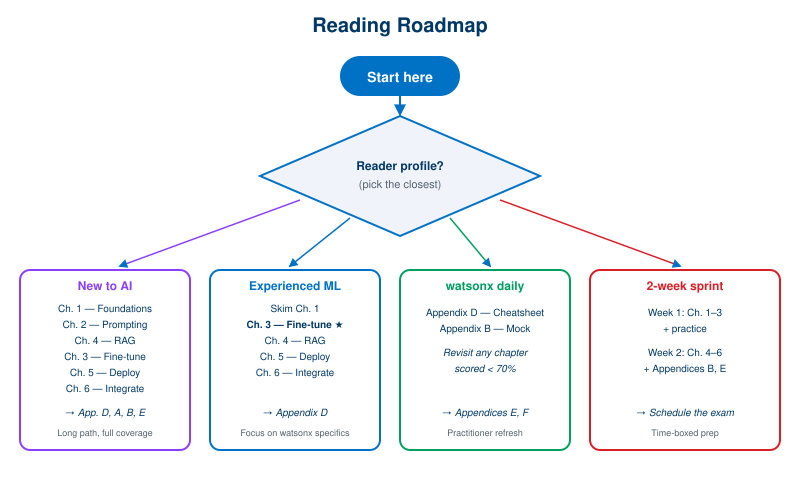
\includegraphics[width=0.95\textwidth]{assets/figures/fig02-roadmap}
\caption{Four suggested reading paths. Pick the closest profile and follow the chapter order in that column.}
\label{fig:roadmap}
\end{figure}

If generative AI is new ground, follow the chapters in order, then read Appendix~D before the first mock. If you have shipped LLMs in production and are here mostly for the watsonx-specific material, skim Chapter~1, deep-read Chapter~3 (it is 31\% of the exam --- spend the time), then move through chapters~4--6 and head straight to the mocks. If you already work on watsonx daily, the cheatsheet plus a first mock will tell you where you actually stand; only re-read chapters where you scored below seventy percent on the mock. For a two-week sprint, take chapters~1--3 in the first week and chapters~4--6 plus both mocks in the second, reviewing only what the mocks flag.

\section*{The exam, in five numbers}

The certification is officially titled \emph{IBM Certified watsonx Generative AI Engineer --- Associate}, exam code \textbf{C1000-185}. It is delivered by Pearson VUE, either at a test centre or online with a proctor, and IBM expects roughly six to twelve months of hands-on watsonx.ai experience before a candidate sits it. The numbers worth memorising fit on one hand: \textbf{sixty-two questions}, \textbf{ninety minutes}, \textbf{forty-four to pass} (about seventy-one percent), \textbf{six sections}, and roughly \textbf{eighty-seven seconds per question} on average. Pacing matters more than raw recall.

\subsection*{Where the points live}

The six exam sections are not equally weighted. Figure~\ref{fig:blueprint} shows them stacked by their share of the test, with the chapter in this book that covers each. Section~3 --- fine-tuning --- is thirty-one percent of the exam, almost a third. That is by design: parameter-efficient fine-tuning (PEFT), LoRA, quantisation, and IBM's InstructLab are the topics IBM most wants candidates to demonstrate, and the chapter ratio in this book is built around that reality.

\begin{figure}[h]
\centering
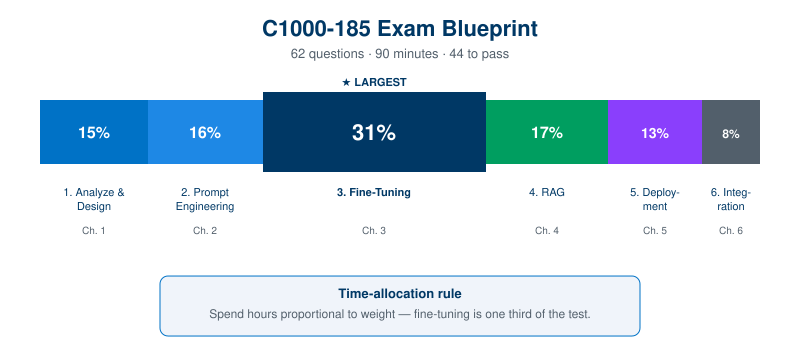
\includegraphics[width=0.95\textwidth]{assets/figures/fig01-exam-blueprint}
\caption{The C1000-185 blueprint at a glance. Section~3 (Fine-Tuning) carries 31\% --- almost a third of the test. Allocate study time in proportion.}
\label{fig:blueprint}
\end{figure}

\examtip{If you take one rule from this preface into your study plan, take this one: \textbf{allocate study hours by section weight, not by comfort}. Fine-tuning is the largest single section, and the section most engineers find least familiar coming in. That gap is exactly where points are won and lost.}

\section*{A thirty-day plan that works}

A month is the right amount of time. Less, and you cram; more, and the first chapters fade before exam day. The plan below front-loads fine-tuning (which earns its 31\% of the exam), uses the back half of week three for the integration material that engineers tend to under-study, and reserves the final week for timed mocks and the cheatsheet. The exact day-count is less important than the rhythm: every week ends with practice questions, not with new material.

\begin{table}[h]
\small
\centering
\begin{tabularx}{\textwidth}{l l X}
\toprule
\textbf{Week} & \textbf{Days} & \textbf{Focus and activities} \\
\midrule
\textbf{Week 1:} & Day 1--2 & \textbf{Foundations}: Chapter~1 (capabilities, patterns, model selection) \\
\textbf{Foundations} & Day 3--5 & \textbf{Prompt engineering}: Chapter~2 (zero/few-shot, parameters, Prompt Lab) \\
& Day 6--7 & \textbf{Review}: practice questions from Chapters~1--2 \\
\midrule
\textbf{Week 2:} & Day 8--12 & \textbf{Fine-tuning}: Chapter~3 (LoRA, quantisation, InstructLab, SDG) --- largest section \\
\textbf{Deep dive} & Day 13--14 & \textbf{Review}: Chapter~3 practice plus a small Tuning Studio job \\
\midrule
\textbf{Week 3:} & Day 15--18 & \textbf{RAG}: Chapter~4 (embeddings, vector DBs, LangChain, agentic RAG) \\
\textbf{Application} & Day 19--21 & \textbf{Deployment}: Chapter~5 (spaces, versioning, gateway) \\
& Day 22--23 & \textbf{Integration}: Chapter~6 (SDK, LangChain, MCP) \\
\midrule
\textbf{Week 4:} & Day 24--26 & \textbf{Comprehensive review}: re-read all Key Takeaways \\
\textbf{Final prep} & Day 27--28 & \textbf{Mock test}: Appendix~B (40 Qs, 60 min) and Appendix~E (longer practice) under timed conditions \\
& Day 29 & \textbf{Mock review}: study weak areas using Appendices~C, F; redo failed questions \\
& Day 30 & \textbf{Final polish}: Cheat Sheet (Appendix~D) plus Glossary (Appendix~A), then rest. \\
\bottomrule
\end{tabularx}
\caption{30-Day study plan.}
\label{tab:study-plan}
\end{table}

\section*{What you should bring to the first page}

This is not a beginner's introduction to machine learning. A working comfort with Python --- enough to read a script, run a notebook, and call a REST API --- is the floor. Some prior exposure to cloud platforms (preferably IBM Cloud, but any major cloud will do) makes the deployment chapter easier. A watsonx.ai account is required for the labs in the companion repository; the free trial covers everything used in this book.

If you have never seen a transformer block, never trained a model, and never written a prompt longer than two sentences, that is fine. The first chapter assumes none of that. What you cannot fake is the rhythm of working code. Read every code listing slowly the first time; the second time, copy it into a notebook and run it.

\section*{Conventions used in this book}

Three typographic rules run through every chapter. \texttt{Monospaced text} is code, file paths, API parameters, and model identifiers (\texttt{ibm/granite-3-2-8b-instruct} is one). \emph{Italics} introduce a new term where it is first defined, and occasionally mark an aside. \textbf{Bold} marks the few words a candidate should be able to recite back from memory.

Coloured boxes appear sparingly. A \textcolor{ibmsuccess}{\textbf{Key Concept}} states a rule worth memorising; an \textcolor{ibmblue}{\textbf{Example}} gives a concrete enterprise scenario; an \textcolor{ibmwarning}{\textbf{Important}} or \textcolor{ibmwarning}{\textbf{Exam Tip}} flags a question pattern the certification uses; a \textcolor{ibmerror}{\textbf{Warning}} marks a pitfall or a deprecated identifier; a \textcolor{ibmgray}{\textbf{Practice Question}} is a self-test with an answer at the end of the chapter. If a chapter ever feels like every paragraph is in a box, that is a bug.

\section*{Acknowledgements}

This book stands on the shoulders of three open-source projects --- InstructLab, LangChain, and LlamaIndex --- whose authors and maintainers deserve more than a paragraph. The publicly available IBM watsonx.ai documentation, written and maintained by an IBM team the author has no commercial relationship with, has been the primary reference for every code listing and model identifier. The readers of the companion YouTube and Udemy courses shaped this edition through their questions; if a section here reads more clearly than the equivalent video, it is because somebody flagged what was muddled.

\vspace{1cm}

\noindent\textit{Good luck on exam day.}

\vspace{0.5cm}

\noindent\textbf{Ruslan Idelfonso Magana Vsevolodovna}\\
\textit{ruslanmv.com}

\cleardoublepage
